% !Mode:: "TeX:UTF-8"
% !TeX program = lualatex

\documentclass[a4paper, 9pt, twocolumn]{extarticle}
\usepackage[dvips]{graphicx}		
\usepackage{tabularx}
\usepackage{multirow}	
\usepackage{url}
%\usepackage[ansinew]{inputenc}
\usepackage{fontspec} %LuaLaTeX
\usepackage{parskip}
\usepackage{amsmath}

% \usepackage[]{auto-pst-pdf}
% \usepackage{pstricks}
 \usepackage{pst-plot}
% \usepackage{pst-node}
% \usepackage{multido}
% \usepackage{url}


\addtolength{\textwidth}{2.1cm}
\addtolength{\topmargin}{-2.4cm}
\addtolength{\oddsidemargin}{-1.1 cm}
\addtolength{\textheight}{4.5cm}
\setlength{\columnsep}{0.7cm}

% User defined macros
\def\x{{\mathbf x}}
\def\L{{\cal L}}
\def\SM{{\mathcal S}}
\def\SMO{{\mathcal S^{\mathrm{chroma}}}}
\def\SMS{{\mathcal S^{\mathrm{enh}}}}
\def\SMP{{\mathcal S^{\mathrm{path}}}}
\def\SMPI{{\mathcal S^{\mathrm{struct}}}}
%\def\SMPC{{\mathcal S^{\mathrm{pc}}}}
\def\SMPC{{\mathcal S^{\mathrm{pb}}}}

\pagestyle{empty}

\begin{document}

\date{\normalsize \today}

\title{\vspace{-8mm}\textbf{\Large
Music Structure Analysis Summary\footnote{This is the summary for the reading assignment,
which is part of the exercise of the lecture \emph{Music Processing Analysis}, Winter Term 2015/16,
Friedrich-Alexander Universit\"at Erlangen-N\"urnberg.
Instructor: Prof.\ Dr.\ Meinard M\"uller,
Tutor: Dipl.-Ing. Stefan Baalke.
}}}

% Hier die Namen und Daten der beteiligten Autoren eintragen
\author{
{
\begin{minipage}[t]{.45\textwidth}
\center
Arnulf Becker\\
\small
Friedrich-Alexander Universit\"at Erlangen-N\"urnberg
\protect\\{} % 
\url{arnulf.becker@FAU.de}
\end{minipage}%
\begin{minipage}[t]{.45\textwidth}
\center
Iñigo Fern\' andez\\%				Iñigo Fernandez\\
\small
Friedrich-Alexander Universit\"at Erlangen-N\"urnberg
\protect\\{} % 
\url{inigo.fernandez@FAU.de}
\end{minipage}%
}
}
 
\maketitle
\thispagestyle{empty}

%%%%%%%%%%%%%%%%%%%%%%%%%%%%%%%%%%%%%%%%%%%%%%%%%%%%%%%%%%%%%%%%%%%%%%%%%%%%%%
\section{Default Introduction [will be removed]}
\label{section:defaultIntroduction}
%%%%%%%%%%%%%%%%%%%%%%%%%%%%%%%%%%%%%%%%%%%%%%%%%%%%%%%%%%%%%%%%%%%%%%%%%%%%%%

This is a \LaTeX-template for the summary of the reading assignment summary. Note that the summary
itself should not exceed one page. Furthermore, please provide your feedback concerning the 
book chapter and the lecture on additional pages.
The style of this template may not be changed.



%%%%%%%%%%%%%%%%%%%%%%%%%%%%%%%%%%%%%%%%%%%%%%%%%%%%%%%%%%%%%%%%%%%%%%%%%%%%%%
\section{Main Section[will be removed]}
\label{section:main}
%%%%%%%%%%%%%%%%%%%%%%%%%%%%%%%%%%%%%%%%%%%%%%%%%%%%%%%%%%%%%%%%%%%%%%%%%%%%%%

The summary should consist of one to three main sections.
Please restrict yourself to describing only the the most
important points covered in the chapter. These sections
should contain the motivation of the problem as well as
the most important technical details. Use an easy to read
language with short, clear sentences. 

%%%%%%%%%%%%%%%%%%%%%%%%%%%%%%%%%%%%%%%%%%%%%%%%%%%%%%%%%%%%%%%%%%%%%%%%%%%%%%
% Here you find some additional LaTex code fragments for including figures and
% references which you may find helpful.
%%%%%%%%%%%%%%%%%%%%%%%%%%%%%%%%%%%%%%%%%%%%%%%%%%%%%%%%%%%%%%%%%%%%%%%%%%%%%%

Example for a citation: \cite{Mueller07_InformationRetrieval_SPRINGER}.

Example for figure: Figure~\ref{figure:example}.

\newpage


\newpage

%%%%%%%%%%%%%%%%%%%%%%%%%%%%%%%%%%%%%%%%%%%%%%%%%%%%%%%%%%%%%%%%%%%%%%%%%%%%%%
\section{General Principles} 
\label{section:generalPrinciples}
%Alternative names: intro, basics...
%%%%%%%%%%%%%%%%%%%%%%%%%%%%%%%%%%%%%%%%%%%%%%%%%%%%%%%%%%%%%%%%%%%%%%%%%%%%%%

\subsection{Musical Structure}  
% Mixture of sections 'intro' and 4.1.2 from the book
The sounds that conform music are not organized in a random way: they are combined conforming musical structures such as phrases, motifs or sections. Those structures are again combined and form higher-level sections that determine the overall layout of the composition, also called \textbf{musical structure}. The names of the mentioned high-level sections may vary depending on the kind of music we are analysing, as well as the way they are arranged. 

\medskip

In Western music, the musical structure often follows certain patterns. The simplest one is the \textbf{strophic form}, which consists of a sequence of a repeated part resulting in a $A_{1}A_{2}A_{3}A_{4}...$ structure, usually used in folk song or nursery rhymes. Medleys or potpourris (concatenation of popular songs) use the so called \textbf{chain form}, a sequence of unrelated parts ($ABCD...$), sometimes with repeats ($A_{1}A_{2}B_{1}B_{2}C_{1}C_{2}...$). Another form is the \textbf{rondo form}, where a recurring theme alternates with contrasting sections $A_{1}BA_{2}CA_{3}DA_{4}...$

\medskip

In Western classical music, one of the most important musical structures is the \textbf{sonata form}. It consists of an \textbf{exposition} ($E$), a \textbf{development} ($D$), and a \textbf{recapitulation} ($R$), where the exposition is repeated once. At a coarse level, that recapitulation can be regarded as a repetition of the exposition, although at a finer level they are different. Sometimes, one can find an additional \textbf{introduction} ($I$) and a closing \textbf{coda} ($C$), thus yielding the form $ IE_{1} E_{2} DRC $. 

\medskip

In popular music, the most typical parts are the \textbf{verse} ($V$ ) and the \textbf{chorus} ($C$)
sections. Each verse usually employs the same melody (possibly with slight modifications), while the lyrics change for each verse. The \textbf{chorus} or \textbf{refrain} typically consists of a melodic and lyrical phrase which is repeated.
Sometimes, pop songs may start with an \textbf{intro} ($I$) and close with an \textbf{outro} ($O$). Finally, verse and chorus sections may be connected by an additional part called a \textbf{bridge} ($B$). The verse and chorus are usually repeated throughout a song, while the intro and the outro appear only once. Some pop songs may also have a \textbf{solo} where an instrument plays a melody. 


\subsection{Structure Analysis and Segmentation}
%from book 4.1.1

goal
basics
different segmentation principles 


\section{Mathematical tools: Self Similarity Matrix}
\label{section:ssm}

\section{Repetition based Segmentation and Audio Thumbnailing}
\label{section:repetition}


\section{Novelty based Segmentation}
\label{section:novelty}

%%%%%%%%%%%%%%%%%%%%%%%%%%%%%%%%%%%%%%%%%%%%%%%%%%%%%%%%%%%%%%%%%%%%%%%%%%%%%%
\section{Feedback}
\label{section:feedback}
%%%%%%%%%%%%%%%%%%%%%%%%%%%%%%%%%%%%%%%%%%%%%%%%%%%%%%%%%%%%%%%%%%%%%%%%%%%%%%


%-----------------------
 \begin{figure}[t]
 \begin{center}
 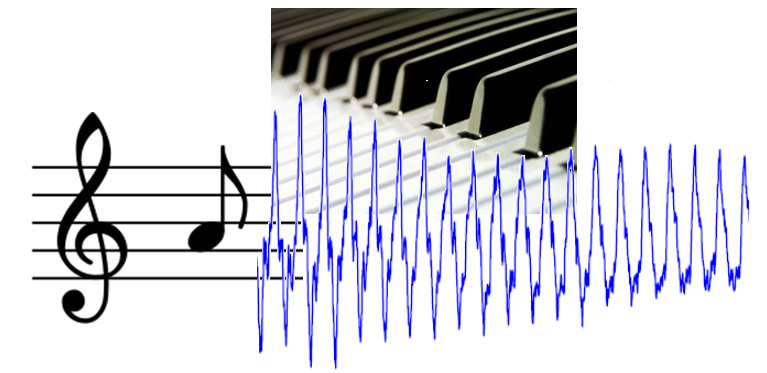
\includegraphics[width=5cm]{figure_example.png}
 \end{center}
 \caption{
 Example for a figure.
 }
 \label{figure:example}
 \end{figure}
%-----------------------


Feedback may also be given in form of bullet points
\begin{itemize}
\item This was good....
\item I did not like...
\end{itemize}



%%%%%%%%%%%%%%%%%%%%%%%%%%%%%%%%%%%%%%%%%%%%%%%%%%%%%%%%%%%%%%%%%%%%%%%%%%%%%%%%%%%%%%%%%%%%%%%%%%
\bibliographystyle{abbrv}
\small
\bibliography{references}
%%%%%%%%%%%%%%%%%%%%%%%%%%%%%%%%%%%%%%%%%%%%%%%%%%%%%%%%%%%%%%%%%%%%%%%%%%%%%%%%%%%%%%%%%%%%%%%%%%



\end{document}

